\documentclass[1p]{elsarticle_modified}
%\bibliographystyle{elsarticle-num}

%\usepackage[colorlinks]{hyperref}
%\usepackage{abbrmath_seonhwa} %\Abb, \Ascr, \Acal ,\Abf, \Afrak
\usepackage{amsfonts}
\usepackage{amssymb}
\usepackage{amsmath}
\usepackage{amsthm}
\usepackage{scalefnt}
\usepackage{amsbsy}
\usepackage{kotex}
\usepackage{caption}
\usepackage{subfig}
\usepackage{color}
\usepackage{graphicx}
\usepackage{xcolor} %% white, black, red, green, blue, cyan, magenta, yellow
\usepackage{float}
\usepackage{setspace}
\usepackage{hyperref}

\usepackage{tikz}
\usetikzlibrary{arrows}

\usepackage{multirow}
\usepackage{array} % fixed length table
\usepackage{hhline}

%%%%%%%%%%%%%%%%%%%%%
\makeatletter
\renewcommand*\env@matrix[1][\arraystretch]{%
	\edef\arraystretch{#1}%
	\hskip -\arraycolsep
	\let\@ifnextchar\new@ifnextchar
	\array{*\c@MaxMatrixCols c}}
\makeatother %https://tex.stackexchange.com/questions/14071/how-can-i-increase-the-line-spacing-in-a-matrix
%%%%%%%%%%%%%%%

\usepackage[normalem]{ulem}

\newcommand{\msout}[1]{\ifmmode\text{\sout{\ensuremath{#1}}}\else\sout{#1}\fi}
%SOURCE: \msout is \stkout macro in https://tex.stackexchange.com/questions/20609/strikeout-in-math-mode

\newcommand{\cancel}[1]{
	\ifmmode
	{\color{red}\msout{#1}}
	\else
	{\color{red}\sout{#1}}
	\fi
}

\newcommand{\add}[1]{
	{\color{blue}\uwave{#1}}
}

\newcommand{\replace}[2]{
	\ifmmode
	{\color{red}\msout{#1}}{\color{blue}\uwave{#2}}
	\else
	{\color{red}\sout{#1}}{\color{blue}\uwave{#2}}
	\fi
}

\newcommand{\Sol}{\mathcal{S}} %segment
\newcommand{\D}{D} %diagram
\newcommand{\A}{\mathcal{A}} %arc


%%%%%%%%%%%%%%%%%%%%%%%%%%%%%5 test

\def\sl{\operatorname{\textup{SL}}(2,\Cbb)}
\def\psl{\operatorname{\textup{PSL}}(2,\Cbb)}
\def\quan{\mkern 1mu \triangleright \mkern 1mu}

\theoremstyle{definition}
\newtheorem{thm}{Theorem}[section]
\newtheorem{prop}[thm]{Proposition}
\newtheorem{lem}[thm]{Lemma}
\newtheorem{ques}[thm]{Question}
\newtheorem{cor}[thm]{Corollary}
\newtheorem{defn}[thm]{Definition}
\newtheorem{exam}[thm]{Example}
\newtheorem{rmk}[thm]{Remark}
\newtheorem{alg}[thm]{Algorithm}

\newcommand{\I}{\sqrt{-1}}
\begin{document}

%\begin{frontmatter}
%
%\title{Boundary parabolic representations of knots up to 8 crossings}
%
%%% Group authors per affiliation:
%\author{Yunhi Cho} 
%\address{Department of Mathematics, University of Seoul, Seoul, Korea}
%\ead{yhcho@uos.ac.kr}
%
%
%\author{Seonhwa Kim} %\fnref{s_kim}}
%\address{Center for Geometry and Physics, Institute for Basic Science, Pohang, 37673, Korea}
%\ead{ryeona17@ibs.re.kr}
%
%\author{Hyuk Kim}
%\address{Department of Mathematical Sciences, Seoul National University, Seoul 08826, Korea}
%\ead{hyukkim@snu.ac.kr}
%
%\author{Seokbeom Yoon}
%\address{Department of Mathematical Sciences, Seoul National University, Seoul, 08826,  Korea}
%\ead{sbyoon15@snu.ac.kr}
%
%\begin{abstract}
%We find all boundary parabolic representation of knots up to 8 crossings.
%
%\end{abstract}
%\begin{keyword}
%    \MSC[2010] 57M25 
%\end{keyword}
%
%\end{frontmatter}

%\linenumbers
%\tableofcontents
%
\newcommand\colored[1]{\textcolor{white}{\rule[-0.35ex]{0.8em}{1.4ex}}\kern-0.8em\color{red} #1}%
%\newcommand\colored[1]{\textcolor{white}{ #1}\kern-2.17ex	\textcolor{white}{ #1}\kern-1.81ex	\textcolor{white}{ #1}\kern-2.15ex\color{red}#1	}

{\Large $\underline{12a_{1178}~(K12a_{1178})}$}

\setlength{\tabcolsep}{10pt}
\renewcommand{\arraystretch}{1.6}
\vspace{1cm}\begin{tabular}{m{100pt}>{\centering\arraybackslash}m{274pt}}
\multirow{5}{120pt}{
	\centering
	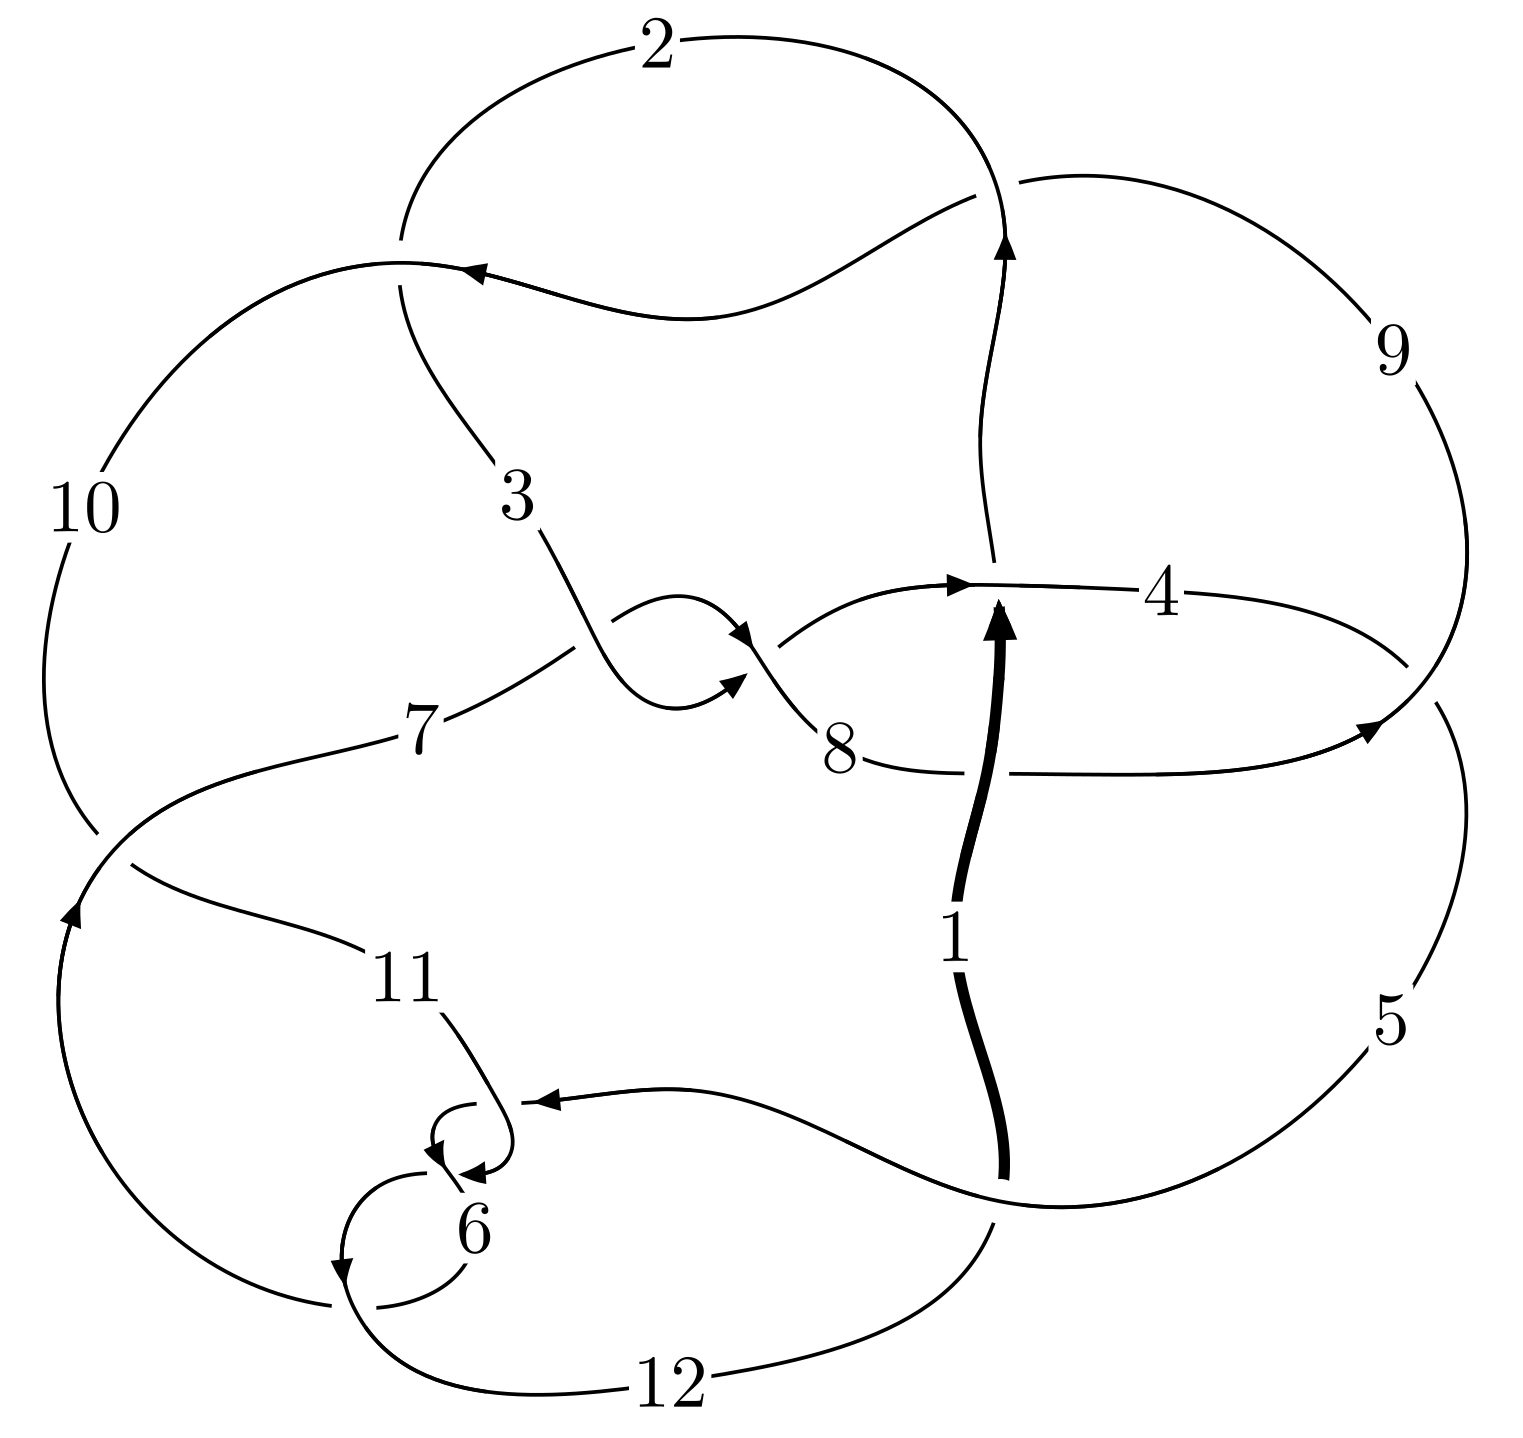
\includegraphics[width=112pt]{../../../GIT/diagram.site/Diagrams/png/1979_12a_1178.png}\\
\ \ \ A knot diagram\footnotemark}&
\allowdisplaybreaks
\textbf{Linearized knot diagam} \\
\cline{2-2}
 &
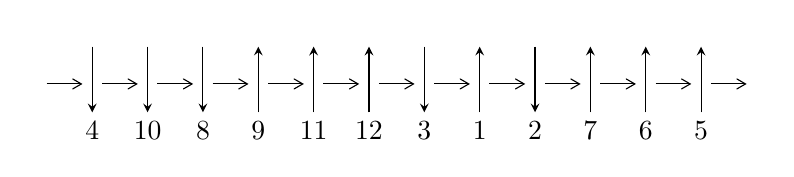
\begin{tikzpicture}[x=20pt, y=17pt]
	% nodes
	\node (C0) at (0, 0) {};
	\node (C1) at (1, 0) {};
	\node (C1U) at (1, +1) {};
	\node (C1D) at (1, -1) {4};

	\node (C2) at (2, 0) {};
	\node (C2U) at (2, +1) {};
	\node (C2D) at (2, -1) {10};

	\node (C3) at (3, 0) {};
	\node (C3U) at (3, +1) {};
	\node (C3D) at (3, -1) {8};

	\node (C4) at (4, 0) {};
	\node (C4U) at (4, +1) {};
	\node (C4D) at (4, -1) {9};

	\node (C5) at (5, 0) {};
	\node (C5U) at (5, +1) {};
	\node (C5D) at (5, -1) {11};

	\node (C6) at (6, 0) {};
	\node (C6U) at (6, +1) {};
	\node (C6D) at (6, -1) {12};

	\node (C7) at (7, 0) {};
	\node (C7U) at (7, +1) {};
	\node (C7D) at (7, -1) {3};

	\node (C8) at (8, 0) {};
	\node (C8U) at (8, +1) {};
	\node (C8D) at (8, -1) {1};

	\node (C9) at (9, 0) {};
	\node (C9U) at (9, +1) {};
	\node (C9D) at (9, -1) {2};

	\node (C10) at (10, 0) {};
	\node (C10U) at (10, +1) {};
	\node (C10D) at (10, -1) {7};

	\node (C11) at (11, 0) {};
	\node (C11U) at (11, +1) {};
	\node (C11D) at (11, -1) {6};

	\node (C12) at (12, 0) {};
	\node (C12U) at (12, +1) {};
	\node (C12D) at (12, -1) {5};
	\node (C13) at (13, 0) {};

	% arrows
	\draw[->,>={angle 60}]
	(C0) edge (C1) (C1) edge (C2) (C2) edge (C3) (C3) edge (C4) (C4) edge (C5) (C5) edge (C6) (C6) edge (C7) (C7) edge (C8) (C8) edge (C9) (C9) edge (C10) (C10) edge (C11) (C11) edge (C12) (C12) edge (C13) ;	\draw[->,>=stealth]
	(C1U) edge (C1D) (C2U) edge (C2D) (C3U) edge (C3D) (C4D) edge (C4U) (C5D) edge (C5U) (C6D) edge (C6U) (C7U) edge (C7D) (C8D) edge (C8U) (C9U) edge (C9D) (C10D) edge (C10U) (C11D) edge (C11U) (C12D) edge (C12U) ;
	\end{tikzpicture} \\
\hhline{~~} \\& 
\textbf{Solving Sequence} \\ \cline{2-2} 
 &
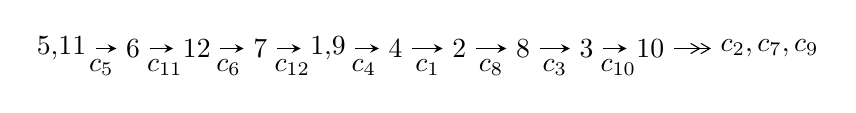
\begin{tikzpicture}[x=23pt, y=7pt]
	% node
	\node (A0) at (-1/8, 0) {5,11};
	\node (A1) at (1, 0) {6};
	\node (A2) at (2, 0) {12};
	\node (A3) at (3, 0) {7};
	\node (A4) at (65/16, 0) {1,9};
	\node (A5) at (41/8, 0) {4};
	\node (A6) at (49/8, 0) {2};
	\node (A7) at (57/8, 0) {8};
	\node (A8) at (65/8, 0) {3};
	\node (A9) at (73/8, 0) {10};
	\node (C1) at (1/2, -1) {$c_{5}$};
	\node (C2) at (3/2, -1) {$c_{11}$};
	\node (C3) at (5/2, -1) {$c_{6}$};
	\node (C4) at (7/2, -1) {$c_{12}$};
	\node (C5) at (37/8, -1) {$c_{4}$};
	\node (C6) at (45/8, -1) {$c_{1}$};
	\node (C7) at (53/8, -1) {$c_{8}$};
	\node (C8) at (61/8, -1) {$c_{3}$};
	\node (C9) at (69/8, -1) {$c_{10}$};
	\node (A10) at (11, 0) {$c_{2},c_{7},c_{9}$};

	% edge
	\draw[->,>=stealth]	
	(A0) edge (A1) (A1) edge (A2) (A2) edge (A3) (A3) edge (A4) (A4) edge (A5) (A5) edge (A6) (A6) edge (A7) (A7) edge (A8) (A8) edge (A9) ;
	\draw[->>,>={angle 60}]	
	(A9) edge (A10);
\end{tikzpicture} \\ 

\end{tabular} \\

\footnotetext{
The image of knot diagram is generated by the software ``\textbf{Draw programme}" developed by Andrew Bartholomew(\url{http://www.layer8.co.uk/maths/draw/index.htm\#Running-draw}), where we modified some parts for our purpose(\url{https://github.com/CATsTAILs/LinksPainter}).
}\phantom \\ \newline 
\centering \textbf{Ideals for irreducible components\footnotemark of $X_{\text{par}}$} 
 
\begin{align*}
I^u_{1}&=\langle 
56 u^{34}+305 u^{33}+\cdots+2 b-284,\;21 u^{34}+135 u^{33}+\cdots+4 a-182,\;u^{35}+7 u^{34}+\cdots+32 u-8\rangle \\
I^u_{2}&=\langle 
3.02051\times10^{26} a^{5} u^{10}+6.10493\times10^{26} a^{4} u^{10}+\cdots+8.97858\times10^{27} a-5.15875\times10^{27},\\
\phantom{I^u_{2}}&\phantom{= \langle  }6 u^{10} a^5+3 u^{10} a^4+\cdots-21 a-22,\;u^{11}- u^{10}-4 u^9+3 u^8+6 u^7-2 u^6-2 u^5-3 u^4-3 u^3+3 u^2+2 u+1\rangle \\
I^u_{3}&=\langle 
u^{20}-9 u^{18}+34 u^{16}-66 u^{14}+59 u^{12}+4 u^{10}+u^9-50 u^8-4 u^7+25 u^6+6 u^5+9 u^4-3 u^3-6 u^2+b,\\
\phantom{I^u_{3}}&\phantom{= \langle  }- u^{19}- u^{18}+\cdots+a+1,\\
\phantom{I^u_{3}}&\phantom{= \langle  }u^{21}-10 u^{19}+42 u^{17}-92 u^{15}+99 u^{13}-14 u^{11}+u^{10}-78 u^9-5 u^8+60 u^7+9 u^6+9 u^5-6 u^4-18 u^3+1\rangle \\
\\
\end{align*}
\raggedright * 3 irreducible components of $\dim_{\mathbb{C}}=0$, with total 122 representations.\\
\footnotetext{All coefficients of polynomials are rational numbers. But the coefficients are sometimes approximated in decimal forms when there is not enough margin.}
\newpage
\renewcommand{\arraystretch}{1}
\centering \section*{I. $I^u_{1}= \langle 56 u^{34}+305 u^{33}+\cdots+2 b-284,\;21 u^{34}+135 u^{33}+\cdots+4 a-182,\;u^{35}+7 u^{34}+\cdots+32 u-8 \rangle$}
\flushleft \textbf{(i) Arc colorings}\\
\begin{tabular}{m{7pt} m{180pt} m{7pt} m{180pt} }
\flushright $a_{5}=$&$\begin{pmatrix}1\\0\end{pmatrix}$ \\
\flushright $a_{11}=$&$\begin{pmatrix}0\\u\end{pmatrix}$ \\
\flushright $a_{6}=$&$\begin{pmatrix}1\\- u^2\end{pmatrix}$ \\
\flushright $a_{12}=$&$\begin{pmatrix}u\\- u^3+u\end{pmatrix}$ \\
\flushright $a_{7}=$&$\begin{pmatrix}- u^2+1\\u^4-2 u^2\end{pmatrix}$ \\
\flushright $a_{1}=$&$\begin{pmatrix}- u^3+2 u\\- u^3+u\end{pmatrix}$ \\
\flushright $a_{9}=$&$\begin{pmatrix}-5.25000 u^{34}-33.7500 u^{33}+\cdots-225.500 u+45.5000\\-28 u^{34}-\frac{305}{2} u^{33}+\cdots-\frac{1307}{2} u+142\end{pmatrix}$ \\
\flushright $a_{4}=$&$\begin{pmatrix}-\frac{75}{2} u^{34}-\frac{855}{4} u^{33}+\cdots-\frac{4301}{4} u+227\\\frac{69}{4} u^{34}+\frac{401}{4} u^{33}+\cdots+560 u-116\end{pmatrix}$ \\
\flushright $a_{2}=$&$\begin{pmatrix}\frac{145}{8} u^{34}+\frac{829}{8} u^{33}+\cdots+551 u-\frac{229}{2}\\-\frac{1}{4} u^{34}-\frac{11}{4} u^{33}+\cdots-\frac{49}{2} u+5\end{pmatrix}$ \\
\flushright $a_{8}=$&$\begin{pmatrix}5.75000 u^{34}+32.2500 u^{33}+\cdots+158.500 u-34.5000\\\frac{53}{2} u^{34}+152 u^{33}+\cdots+\frac{1537}{2} u-162\end{pmatrix}$ \\
\flushright $a_{3}=$&$\begin{pmatrix}-\frac{47}{8} u^{34}-\frac{291}{8} u^{33}+\cdots-232 u+\frac{95}{2}\\\frac{67}{4} u^{34}+\frac{369}{4} u^{33}+\cdots+\frac{877}{2} u-93\end{pmatrix}$ \\
\flushright $a_{10}=$&$\begin{pmatrix}- u^5+2 u^3- u\\u^7-3 u^5+2 u^3+u\end{pmatrix}$\\&\end{tabular}
\flushleft \textbf{(ii) Obstruction class $= -1$}\\~\\
\flushleft \textbf{(iii) Cusp Shapes $= -14 u^{34}-83 u^{33}-49 u^{32}+552 u^{31}+749 u^{30}-1851 u^{29}-2942 u^{28}+4360 u^{27}+5628 u^{26}-8667 u^{25}-3703 u^{24}+14324 u^{23}-8289 u^{22}-14914 u^{21}+26100 u^{20}-98 u^{19}-31837 u^{18}+26886 u^{17}+11105 u^{16}-37472 u^{15}+22359 u^{14}+14556 u^{13}-32711 u^{12}+16400 u^{11}+10929 u^{10}-19848 u^9+10674 u^8+3645 u^7-8028 u^6+5365 u^5-279 u^4-1570 u^3+1326 u^2-556 u+122$}\\~\\
\newpage\renewcommand{\arraystretch}{1}
\flushleft \textbf{(iv) u-Polynomials at the component}\newline \\
\begin{tabular}{m{50pt}|m{274pt}}
Crossings & \hspace{64pt}u-Polynomials at each crossing \\
\hline $$\begin{aligned}c_{1}\end{aligned}$$&$\begin{aligned}
&u^{35}-33 u^{34}+\cdots-40960 u+2048
\end{aligned}$\\
\hline $$\begin{aligned}c_{2},c_{3},c_{7}\\c_{9}\end{aligned}$$&$\begin{aligned}
&u^{35}- u^{34}+\cdots+u-1
\end{aligned}$\\
\hline $$\begin{aligned}c_{4},c_{8}\end{aligned}$$&$\begin{aligned}
&u^{35}+6 u^{33}+\cdots+2 u-1
\end{aligned}$\\
\hline $$\begin{aligned}c_{5},c_{6},c_{11}\end{aligned}$$&$\begin{aligned}
&u^{35}+7 u^{34}+\cdots+32 u-8
\end{aligned}$\\
\hline $$\begin{aligned}c_{10},c_{12}\end{aligned}$$&$\begin{aligned}
&u^{35}-21 u^{34}+\cdots-40656 u+2664
\end{aligned}$\\
\hline
\end{tabular}\\~\\
\newpage\renewcommand{\arraystretch}{1}
\flushleft \textbf{(v) Riley Polynomials at the component}\newline \\
\begin{tabular}{m{50pt}|m{274pt}}
Crossings & \hspace{64pt}Riley Polynomials at each crossing \\
\hline $$\begin{aligned}c_{1}\end{aligned}$$&$\begin{aligned}
&y^{35}-11 y^{34}+\cdots+14680064 y-4194304
\end{aligned}$\\
\hline $$\begin{aligned}c_{2},c_{3},c_{7}\\c_{9}\end{aligned}$$&$\begin{aligned}
&y^{35}-35 y^{34}+\cdots-17 y-1
\end{aligned}$\\
\hline $$\begin{aligned}c_{4},c_{8}\end{aligned}$$&$\begin{aligned}
&y^{35}+12 y^{34}+\cdots+12 y-1
\end{aligned}$\\
\hline $$\begin{aligned}c_{5},c_{6},c_{11}\end{aligned}$$&$\begin{aligned}
&y^{35}-29 y^{34}+\cdots+32 y-64
\end{aligned}$\\
\hline $$\begin{aligned}c_{10},c_{12}\end{aligned}$$&$\begin{aligned}
&y^{35}+23 y^{34}+\cdots+27880992 y-7096896
\end{aligned}$\\
\hline
\end{tabular}\\~\\
\newpage\flushleft \textbf{(vi) Complex Volumes and Cusp Shapes}
$$\begin{array}{c|c|c}  
\text{Solutions to }I^u_{1}& \I (\text{vol} + \sqrt{-1}CS) & \text{Cusp shape}\\
 \hline 
\begin{aligned}
u &= \phantom{-}0.139537 + 0.931995 I \\
a &= -0.469976 + 1.183650 I \\
b &= \phantom{-}0.039825 + 0.846776 I\end{aligned}
 & -12.11410 + 3.47580 I & -9.19807 - 3.18333 I \\ \hline\begin{aligned}
u &= \phantom{-}0.139537 - 0.931995 I \\
a &= -0.469976 - 1.183650 I \\
b &= \phantom{-}0.039825 - 0.846776 I\end{aligned}
 & -12.11410 - 3.47580 I & -9.19807 + 3.18333 I \\ \hline\begin{aligned}
u &= \phantom{-}0.105864 + 0.897053 I \\
a &= \phantom{-}0.44787 + 2.53244 I \\
b &= \phantom{-}0.94342 + 1.35103 I\end{aligned}
 & -13.7151 + 12.5847 I & -5.18347 - 6.53919 I \\ \hline\begin{aligned}
u &= \phantom{-}0.105864 - 0.897053 I \\
a &= \phantom{-}0.44787 - 2.53244 I \\
b &= \phantom{-}0.94342 - 1.35103 I\end{aligned}
 & -13.7151 - 12.5847 I & -5.18347 + 6.53919 I \\ \hline\begin{aligned}
u &= \phantom{-}0.636350 + 0.611239 I \\
a &= \phantom{-}0.942619 - 0.315270 I \\
b &= \phantom{-}0.574414 - 0.905738 I\end{aligned}
 & -6.32739 - 3.08954 I & -4.56075 + 2.58207 I \\ \hline\begin{aligned}
u &= \phantom{-}0.636350 - 0.611239 I \\
a &= \phantom{-}0.942619 + 0.315270 I \\
b &= \phantom{-}0.574414 + 0.905738 I\end{aligned}
 & -6.32739 + 3.08954 I & -4.56075 - 2.58207 I \\ \hline\begin{aligned}
u &= \phantom{-}0.472041 + 0.666318 I \\
a &= \phantom{-}0.12197 - 1.43044 I \\
b &= -0.746358 - 1.022450 I\end{aligned}
 & -6.79949 + 7.60511 I & -4.01817 - 7.64944 I \\ \hline\begin{aligned}
u &= \phantom{-}0.472041 - 0.666318 I \\
a &= \phantom{-}0.12197 + 1.43044 I \\
b &= -0.746358 + 1.022450 I\end{aligned}
 & -6.79949 - 7.60511 I & -4.01817 + 7.64944 I \\ \hline\begin{aligned}
u &= \phantom{-}1.179240 + 0.305684 I \\
a &= \phantom{-}0.513879 - 0.597102 I \\
b &= \phantom{-}0.558931 - 1.032860 I\end{aligned}
 & \phantom{-}0.229089 + 0.656619 I & \phantom{-}3.86417 - 1.98226 I \\ \hline\begin{aligned}
u &= \phantom{-}1.179240 - 0.305684 I \\
a &= \phantom{-}0.513879 + 0.597102 I \\
b &= \phantom{-}0.558931 + 1.032860 I\end{aligned}
 & \phantom{-}0.229089 - 0.656619 I & \phantom{-}3.86417 + 1.98226 I\\
 \hline 
 \end{array}$$\newpage$$\begin{array}{c|c|c}  
\text{Solutions to }I^u_{1}& \I (\text{vol} + \sqrt{-1}CS) & \text{Cusp shape}\\
 \hline 
\begin{aligned}
u &= \phantom{-}0.088955 + 0.772136 I \\
a &= -0.26673 - 2.09268 I \\
b &= -0.755605 - 0.993491 I\end{aligned}
 & -3.07455 + 3.26826 I & \phantom{-}1.60586 - 2.42356 I \\ \hline\begin{aligned}
u &= \phantom{-}0.088955 - 0.772136 I \\
a &= -0.26673 + 2.09268 I \\
b &= -0.755605 + 0.993491 I\end{aligned}
 & -3.07455 - 3.26826 I & \phantom{-}1.60586 + 2.42356 I \\ \hline\begin{aligned}
u &= \phantom{-}1.139170 + 0.518187 I \\
a &= -0.127484 + 0.654094 I \\
b &= \phantom{-}0.098871 + 0.884816 I\end{aligned}
 & -9.05046 + 1.64505 I & -6.82659 - 2.03985 I \\ \hline\begin{aligned}
u &= \phantom{-}1.139170 - 0.518187 I \\
a &= -0.127484 - 0.654094 I \\
b &= \phantom{-}0.098871 - 0.884816 I\end{aligned}
 & -9.05046 - 1.64505 I & -6.82659 + 2.03985 I \\ \hline\begin{aligned}
u &= \phantom{-}1.174450 + 0.465803 I \\
a &= -0.882414 + 0.762013 I \\
b &= -0.88026 + 1.32953 I\end{aligned}
 & -10.43630 - 7.73132 I & -2.52329 + 3.10208 I \\ \hline\begin{aligned}
u &= \phantom{-}1.174450 - 0.465803 I \\
a &= -0.882414 - 0.762013 I \\
b &= -0.88026 - 1.32953 I\end{aligned}
 & -10.43630 + 7.73132 I & -2.52329 - 3.10208 I \\ \hline\begin{aligned}
u &= -1.299980 + 0.228637 I \\
a &= -0.285197 - 1.010500 I \\
b &= \phantom{-}0.690456 - 0.023660 I\end{aligned}
 & \phantom{-}4.00950 - 4.24760 I & \phantom{-}7.23862 + 6.55308 I \\ \hline\begin{aligned}
u &= -1.299980 - 0.228637 I \\
a &= -0.285197 + 1.010500 I \\
b &= \phantom{-}0.690456 + 0.023660 I\end{aligned}
 & \phantom{-}4.00950 + 4.24760 I & \phantom{-}7.23862 - 6.55308 I \\ \hline\begin{aligned}
u &= \phantom{-}1.32721\phantom{ +0.000000I} \\
a &= \phantom{-}0.210158\phantom{ +0.000000I} \\
b &= \phantom{-}0.310775\phantom{ +0.000000I}\end{aligned}
 & \phantom{-}2.90599\phantom{ +0.000000I} & \phantom{-}1.01730\phantom{ +0.000000I} \\ \hline\begin{aligned}
u &= -1.337390 + 0.048424 I \\
a &= \phantom{-}1.165230 - 0.179093 I \\
b &= -0.857438 + 0.443510 I\end{aligned}
 & \phantom{-}6.13792 - 1.57371 I & \phantom{-}10.75089 + 1.90988 I\\
 \hline 
 \end{array}$$\newpage$$\begin{array}{c|c|c}  
\text{Solutions to }I^u_{1}& \I (\text{vol} + \sqrt{-1}CS) & \text{Cusp shape}\\
 \hline 
\begin{aligned}
u &= -1.337390 - 0.048424 I \\
a &= \phantom{-}1.165230 + 0.179093 I \\
b &= -0.857438 - 0.443510 I\end{aligned}
 & \phantom{-}6.13792 + 1.57371 I & \phantom{-}10.75089 - 1.90988 I \\ \hline\begin{aligned}
u &= -1.322170 + 0.332092 I \\
a &= -1.14041 - 1.41439 I \\
b &= \phantom{-}0.885409 - 0.964095 I\end{aligned}
 & \phantom{-}1.35102 - 7.25772 I & \phantom{-}7.15814 + 5.17869 I \\ \hline\begin{aligned}
u &= -1.322170 - 0.332092 I \\
a &= -1.14041 + 1.41439 I \\
b &= \phantom{-}0.885409 + 0.964095 I\end{aligned}
 & \phantom{-}1.35102 + 7.25772 I & \phantom{-}7.15814 - 5.17869 I \\ \hline\begin{aligned}
u &= -1.350510 + 0.404254 I \\
a &= \phantom{-}1.18027 + 1.81624 I \\
b &= -0.99393 + 1.35081 I\end{aligned}
 & -9.1437 - 17.2482 I & \phantom{-0.000000 -}0. + 8.79521 I \\ \hline\begin{aligned}
u &= -1.350510 - 0.404254 I \\
a &= \phantom{-}1.18027 - 1.81624 I \\
b &= -0.99393 - 1.35081 I\end{aligned}
 & -9.1437 + 17.2482 I & \phantom{-0.000000 } 0. - 8.79521 I \\ \hline\begin{aligned}
u &= -1.37576 + 0.42280 I \\
a &= \phantom{-}0.814461 + 0.541541 I \\
b &= -0.138556 + 0.789658 I\end{aligned}
 & -7.35335 - 8.32792 I & \phantom{-0.000000 } 0 \\ \hline\begin{aligned}
u &= -1.37576 - 0.42280 I \\
a &= \phantom{-}0.814461 - 0.541541 I \\
b &= -0.138556 - 0.789658 I\end{aligned}
 & -7.35335 + 8.32792 I & \phantom{-0.000000 } 0 \\ \hline\begin{aligned}
u &= -1.42904 + 0.19328 I \\
a &= -1.014210 - 0.478584 I \\
b &= \phantom{-}0.934761 - 1.000360 I\end{aligned}
 & -0.66389 - 10.53050 I & \phantom{-0.000000 -}0. + 8.08764 I \\ \hline\begin{aligned}
u &= -1.42904 - 0.19328 I \\
a &= -1.014210 + 0.478584 I \\
b &= \phantom{-}0.934761 + 1.000360 I\end{aligned}
 & -0.66389 + 10.53050 I & \phantom{-0.000000 } 0. - 8.08764 I \\ \hline\begin{aligned}
u &= \phantom{-}0.115996 + 0.532001 I \\
a &= -0.741619 - 0.675829 I \\
b &= -0.507252 + 0.043187 I\end{aligned}
 & -0.37214 + 1.40883 I & \phantom{-}0.98492 - 6.02743 I\\
 \hline 
 \end{array}$$\newpage$$\begin{array}{c|c|c}  
\text{Solutions to }I^u_{1}& \I (\text{vol} + \sqrt{-1}CS) & \text{Cusp shape}\\
 \hline 
\begin{aligned}
u &= \phantom{-}0.115996 - 0.532001 I \\
a &= -0.741619 + 0.675829 I \\
b &= -0.507252 - 0.043187 I\end{aligned}
 & -0.37214 - 1.40883 I & \phantom{-}0.98492 + 6.02743 I \\ \hline\begin{aligned}
u &= -1.50719 + 0.09928 I \\
a &= -0.073091 + 0.314181 I \\
b &= -0.521031 - 0.600961 I\end{aligned}
 & \phantom{-}0.874150 + 0.821107 I & \phantom{-0.000000 } 0 \\ \hline\begin{aligned}
u &= -1.50719 - 0.09928 I \\
a &= -0.073091 - 0.314181 I \\
b &= -0.521031 + 0.600961 I\end{aligned}
 & \phantom{-}0.874150 - 0.821107 I & \phantom{-0.000000 } 0 \\ \hline\begin{aligned}
u &= \phantom{-}0.406834 + 0.217699 I \\
a &= -0.540240 + 0.373595 I \\
b &= \phantom{-}0.518952 + 0.467501 I\end{aligned}
 & \phantom{-}0.843371 + 0.754361 I & \phantom{-}6.99963 - 3.56017 I \\ \hline\begin{aligned}
u &= \phantom{-}0.406834 - 0.217699 I \\
a &= -0.540240 - 0.373595 I \\
b &= \phantom{-}0.518952 - 0.467501 I\end{aligned}
 & \phantom{-}0.843371 - 0.754361 I & \phantom{-}6.99963 + 3.56017 I\\
 \hline 
 \end{array}$$\newpage\newpage\renewcommand{\arraystretch}{1}
\centering \section*{II. $I^u_{2}= \langle 3.02\times10^{26} a^{5} u^{10}+6.10\times10^{26} a^{4} u^{10}+\cdots+8.98\times10^{27} a-5.16\times10^{27},\;6 u^{10} a^5+3 u^{10} a^4+\cdots-21 a-22,\;u^{11}- u^{10}+\cdots+2 u+1 \rangle$}
\flushleft \textbf{(i) Arc colorings}\\
\begin{tabular}{m{7pt} m{180pt} m{7pt} m{180pt} }
\flushright $a_{5}=$&$\begin{pmatrix}1\\0\end{pmatrix}$ \\
\flushright $a_{11}=$&$\begin{pmatrix}0\\u\end{pmatrix}$ \\
\flushright $a_{6}=$&$\begin{pmatrix}1\\- u^2\end{pmatrix}$ \\
\flushright $a_{12}=$&$\begin{pmatrix}u\\- u^3+u\end{pmatrix}$ \\
\flushright $a_{7}=$&$\begin{pmatrix}- u^2+1\\u^4-2 u^2\end{pmatrix}$ \\
\flushright $a_{1}=$&$\begin{pmatrix}- u^3+2 u\\- u^3+u\end{pmatrix}$ \\
\flushright $a_{9}=$&$\begin{pmatrix}a\\-0.268598 a^{5} u^{10}-0.542878 a^{4} u^{10}+\cdots-7.98417 a+4.58740\end{pmatrix}$ \\
\flushright $a_{4}=$&$\begin{pmatrix}0.321036 a^{5} u^{10}-0.325338 a^{4} u^{10}+\cdots-7.53353 a-3.76774\\-0.0259755 a^{5} u^{10}+0.100771 a^{4} u^{10}+\cdots-12.9385 a-4.93938\end{pmatrix}$ \\
\flushright $a_{2}=$&$\begin{pmatrix}-0.189655 a^{5} u^{10}+0.295091 a^{4} u^{10}+\cdots+3.91116 a-1.41976\\0.214494 a^{5} u^{10}-0.0282051 a^{4} u^{10}+\cdots-1.53483 a+1.62382\end{pmatrix}$ \\
\flushright $a_{8}=$&$\begin{pmatrix}-0.0275683 a^{5} u^{10}+0.636168 a^{4} u^{10}+\cdots+7.09030 a+1.91159\\-0.441675 a^{5} u^{10}-0.266441 a^{4} u^{10}+\cdots-6.09828 a+5.22750\end{pmatrix}$ \\
\flushright $a_{3}=$&$\begin{pmatrix}-0.0475459 a^{5} u^{10}+0.162203 a^{4} u^{10}+\cdots+4.46863 a-1.45142\\0.172998 a^{5} u^{10}-0.210633 a^{4} u^{10}+\cdots-1.90938 a+2.02365\end{pmatrix}$ \\
\flushright $a_{10}=$&$\begin{pmatrix}- u^5+2 u^3- u\\u^7-3 u^5+2 u^3+u\end{pmatrix}$\\&\end{tabular}
\flushleft \textbf{(ii) Obstruction class $= -1$}\\~\\
\flushleft \textbf{(iii) Cusp Shapes $= -\frac{504039224100025701115835624}{374849606289697770228372931} u^{10} a^5-\frac{1172155967916274982800424384}{374849606289697770228372931} u^{10} a^4+\cdots-\frac{5075735830037470664374767476}{374849606289697770228372931} a+\frac{9670853239799093529630437046}{374849606289697770228372931}$}\\~\\
\newpage\renewcommand{\arraystretch}{1}
\flushleft \textbf{(iv) u-Polynomials at the component}\newline \\
\begin{tabular}{m{50pt}|m{274pt}}
Crossings & \hspace{64pt}u-Polynomials at each crossing \\
\hline $$\begin{aligned}c_{1}\end{aligned}$$&$\begin{aligned}
&(u^3+u^2-1)^{22}
\end{aligned}$\\
\hline $$\begin{aligned}c_{2},c_{3},c_{7}\\c_{9}\end{aligned}$$&$\begin{aligned}
&u^{66}+u^{65}+\cdots+16520 u-4657
\end{aligned}$\\
\hline $$\begin{aligned}c_{4},c_{8}\end{aligned}$$&$\begin{aligned}
&u^{66}+3 u^{65}+\cdots-4900 u-599
\end{aligned}$\\
\hline $$\begin{aligned}c_{5},c_{6},c_{11}\end{aligned}$$&$\begin{aligned}
&(u^{11}- u^{10}-4 u^9+3 u^8+6 u^7-2 u^6-2 u^5-3 u^4-3 u^3+3 u^2+2 u+1)^6
\end{aligned}$\\
\hline $$\begin{aligned}c_{10},c_{12}\end{aligned}$$&$\begin{aligned}
&(u^{11}+3 u^{10}+\cdots-2 u-1)^{6}
\end{aligned}$\\
\hline
\end{tabular}\\~\\
\newpage\renewcommand{\arraystretch}{1}
\flushleft \textbf{(v) Riley Polynomials at the component}\newline \\
\begin{tabular}{m{50pt}|m{274pt}}
Crossings & \hspace{64pt}Riley Polynomials at each crossing \\
\hline $$\begin{aligned}c_{1}\end{aligned}$$&$\begin{aligned}
&(y^3- y^2+2 y-1)^{22}
\end{aligned}$\\
\hline $$\begin{aligned}c_{2},c_{3},c_{7}\\c_{9}\end{aligned}$$&$\begin{aligned}
&y^{66}-57 y^{65}+\cdots+855089512 y+21687649
\end{aligned}$\\
\hline $$\begin{aligned}c_{4},c_{8}\end{aligned}$$&$\begin{aligned}
&y^{66}+19 y^{65}+\cdots+9965280 y+358801
\end{aligned}$\\
\hline $$\begin{aligned}c_{5},c_{6},c_{11}\end{aligned}$$&$\begin{aligned}
&(y^{11}-9 y^{10}+\cdots-2 y-1)^{6}
\end{aligned}$\\
\hline $$\begin{aligned}c_{10},c_{12}\end{aligned}$$&$\begin{aligned}
&(y^{11}+11 y^{10}+\cdots+6 y-1)^{6}
\end{aligned}$\\
\hline
\end{tabular}\\~\\
\newpage\flushleft \textbf{(vi) Complex Volumes and Cusp Shapes}
$$\begin{array}{c|c|c}  
\text{Solutions to }I^u_{2}& \I (\text{vol} + \sqrt{-1}CS) & \text{Cusp shape}\\
 \hline 
\begin{aligned}
u &= -1.14725\phantom{ +0.000000I} \\
a &= -0.681685 + 0.142265 I \\
b &= -0.203831 - 1.332020 I\end{aligned}
 & \phantom{-}0.28470 + 2.82812 I & -0.86650 - 2.97945 I \\ \hline\begin{aligned}
u &= -1.14725\phantom{ +0.000000I} \\
a &= -0.681685 - 0.142265 I \\
b &= -0.203831 + 1.332020 I\end{aligned}
 & \phantom{-}0.28470 - 2.82812 I & -0.86650 + 2.97945 I \\ \hline\begin{aligned}
u &= -1.14725\phantom{ +0.000000I} \\
a &= -0.31870 + 1.52370 I \\
b &= \phantom{-}0.407188 + 0.993368 I\end{aligned}
 & \phantom{-}0.28470 + 2.82812 I & -0.86650 - 2.97945 I \\ \hline\begin{aligned}
u &= -1.14725\phantom{ +0.000000I} \\
a &= -0.31870 - 1.52370 I \\
b &= \phantom{-}0.407188 - 0.993368 I\end{aligned}
 & \phantom{-}0.28470 - 2.82812 I & -0.86650 + 2.97945 I \\ \hline\begin{aligned}
u &= -1.14725\phantom{ +0.000000I} \\
a &= -2.88593\phantom{ +0.000000I} \\
b &= \phantom{-}1.63935\phantom{ +0.000000I}\end{aligned}
 & -3.85288\phantom{ +0.000000I} & -7.39580\phantom{ +0.000000I} \\ \hline\begin{aligned}
u &= -1.14725\phantom{ +0.000000I} \\
a &= -4.00191\phantom{ +0.000000I} \\
b &= -0.239197\phantom{ +0.000000I}\end{aligned}
 & -3.85288\phantom{ +0.000000I} & -7.39580\phantom{ +0.000000I} \\ \hline\begin{aligned}
u &= -0.044199 + 0.849205 I \\
a &= \phantom{-}0.72801 - 1.52143 I \\
b &= \phantom{-}0.825388 - 0.962313 I\end{aligned}
 & -7.55328 - 0.21340 I & -4.55146 - 0.15703 I \\ \hline\begin{aligned}
u &= -0.044199 + 0.849205 I \\
a &= \phantom{-}0.65416 + 1.77567 I \\
b &= -0.047317 + 0.807179 I\end{aligned}
 & -7.55328 - 0.21340 I & -4.55146 - 0.15703 I \\ \hline\begin{aligned}
u &= -0.044199 + 0.849205 I \\
a &= \phantom{-}0.00071 - 2.02802 I \\
b &= \phantom{-}0.774141 - 0.907919 I\end{aligned}
 & -7.55328 - 5.86965 I & -4.55146 + 5.80187 I \\ \hline\begin{aligned}
u &= -0.044199 + 0.849205 I \\
a &= -0.67415 + 2.52234 I \\
b &= \phantom{-}0.057490 + 0.752723 I\end{aligned}
 & -11.69090 - 3.04152 I & -11.08072 + 2.82242 I\\
 \hline 
 \end{array}$$\newpage$$\begin{array}{c|c|c}  
\text{Solutions to }I^u_{2}& \I (\text{vol} + \sqrt{-1}CS) & \text{Cusp shape}\\
 \hline 
\begin{aligned}
u &= -0.044199 + 0.849205 I \\
a &= \phantom{-}2.42363 + 2.14160 I \\
b &= \phantom{-}1.83368 + 1.32855 I\end{aligned}
 & -11.69090 - 3.04152 I & -11.08072 + 2.82242 I \\ \hline\begin{aligned}
u &= -0.044199 + 0.849205 I \\
a &= -0.87468 + 3.12856 I \\
b &= -1.00287 + 1.66762 I\end{aligned}
 & -7.55328 - 5.86965 I & -4.55146 + 5.80187 I \\ \hline\begin{aligned}
u &= -0.044199 - 0.849205 I \\
a &= \phantom{-}0.72801 + 1.52143 I \\
b &= \phantom{-}0.825388 + 0.962313 I\end{aligned}
 & -7.55328 + 0.21340 I & -4.55146 + 0.15703 I \\ \hline\begin{aligned}
u &= -0.044199 - 0.849205 I \\
a &= \phantom{-}0.65416 - 1.77567 I \\
b &= -0.047317 - 0.807179 I\end{aligned}
 & -7.55328 + 0.21340 I & -4.55146 + 0.15703 I \\ \hline\begin{aligned}
u &= -0.044199 - 0.849205 I \\
a &= \phantom{-}0.00071 + 2.02802 I \\
b &= \phantom{-}0.774141 + 0.907919 I\end{aligned}
 & -7.55328 + 5.86965 I & -4.55146 - 5.80187 I \\ \hline\begin{aligned}
u &= -0.044199 - 0.849205 I \\
a &= -0.67415 - 2.52234 I \\
b &= \phantom{-}0.057490 - 0.752723 I\end{aligned}
 & -11.69090 + 3.04152 I & -11.08072 - 2.82242 I \\ \hline\begin{aligned}
u &= -0.044199 - 0.849205 I \\
a &= \phantom{-}2.42363 - 2.14160 I \\
b &= \phantom{-}1.83368 - 1.32855 I\end{aligned}
 & -11.69090 + 3.04152 I & -11.08072 - 2.82242 I \\ \hline\begin{aligned}
u &= -0.044199 - 0.849205 I \\
a &= -0.87468 - 3.12856 I \\
b &= -1.00287 - 1.66762 I\end{aligned}
 & -7.55328 + 5.86965 I & -4.55146 - 5.80187 I \\ \hline\begin{aligned}
u &= -1.232090 + 0.392876 I \\
a &= -0.001588 + 1.162910 I \\
b &= -0.022577 + 0.868095 I\end{aligned}
 & -3.88773 - 4.24511 I & -1.28155 + 3.61318 I \\ \hline\begin{aligned}
u &= -1.232090 + 0.392876 I \\
a &= -0.787317 - 0.081147 I \\
b &= -0.708436 - 1.070380 I\end{aligned}
 & -3.88773 - 4.24511 I & -1.28155 + 3.61318 I\\
 \hline 
 \end{array}$$\newpage$$\begin{array}{c|c|c}  
\text{Solutions to }I^u_{2}& \I (\text{vol} + \sqrt{-1}CS) & \text{Cusp shape}\\
 \hline 
\begin{aligned}
u &= -1.232090 + 0.392876 I \\
a &= -0.113083 - 0.696667 I \\
b &= -0.730235 - 0.947386 I\end{aligned}
 & -3.88773 + 1.41114 I & -1.28155 - 2.34572 I \\ \hline\begin{aligned}
u &= -1.232090 + 0.392876 I \\
a &= \phantom{-}1.43869 + 0.88464 I \\
b &= \phantom{-}0.89523 + 1.68771 I\end{aligned}
 & -3.88773 + 1.41114 I & -1.28155 - 2.34572 I \\ \hline\begin{aligned}
u &= -1.232090 + 0.392876 I \\
a &= \phantom{-}1.52441 + 1.86194 I \\
b &= -0.055694 + 0.670879 I\end{aligned}
 & -8.02531 - 1.41699 I & -7.81082 + 0.63373 I \\ \hline\begin{aligned}
u &= -1.232090 + 0.392876 I \\
a &= \phantom{-}0.32325 + 2.50924 I \\
b &= -1.89288 + 1.18137 I\end{aligned}
 & -8.02531 - 1.41699 I & -7.81082 + 0.63373 I \\ \hline\begin{aligned}
u &= -1.232090 - 0.392876 I \\
a &= -0.001588 - 1.162910 I \\
b &= -0.022577 - 0.868095 I\end{aligned}
 & -3.88773 + 4.24511 I & -1.28155 - 3.61318 I \\ \hline\begin{aligned}
u &= -1.232090 - 0.392876 I \\
a &= -0.787317 + 0.081147 I \\
b &= -0.708436 + 1.070380 I\end{aligned}
 & -3.88773 + 4.24511 I & -1.28155 - 3.61318 I \\ \hline\begin{aligned}
u &= -1.232090 - 0.392876 I \\
a &= -0.113083 + 0.696667 I \\
b &= -0.730235 + 0.947386 I\end{aligned}
 & -3.88773 - 1.41114 I & -1.28155 + 2.34572 I \\ \hline\begin{aligned}
u &= -1.232090 - 0.392876 I \\
a &= \phantom{-}1.43869 - 0.88464 I \\
b &= \phantom{-}0.89523 - 1.68771 I\end{aligned}
 & -3.88773 - 1.41114 I & -1.28155 + 2.34572 I \\ \hline\begin{aligned}
u &= -1.232090 - 0.392876 I \\
a &= \phantom{-}1.52441 - 1.86194 I \\
b &= -0.055694 - 0.670879 I\end{aligned}
 & -8.02531 + 1.41699 I & -7.81082 - 0.63373 I \\ \hline\begin{aligned}
u &= -1.232090 - 0.392876 I \\
a &= \phantom{-}0.32325 - 2.50924 I \\
b &= -1.89288 - 1.18137 I\end{aligned}
 & -8.02531 + 1.41699 I & -7.81082 - 0.63373 I\\
 \hline 
 \end{array}$$\newpage$$\begin{array}{c|c|c}  
\text{Solutions to }I^u_{2}& \I (\text{vol} + \sqrt{-1}CS) & \text{Cusp shape}\\
 \hline 
\begin{aligned}
u &= \phantom{-}1.317220 + 0.129556 I \\
a &= \phantom{-}0.357508 - 0.783708 I \\
b &= -0.127941 + 0.198219 I\end{aligned}
 & \phantom{-}3.27094 + 0.11860 I & \phantom{-}5.30912 - 1.13842 I \\ \hline\begin{aligned}
u &= \phantom{-}1.317220 + 0.129556 I \\
a &= \phantom{-}0.091337 + 0.694344 I \\
b &= \phantom{-}0.776455 - 0.377674 I\end{aligned}
 & \phantom{-}3.27094 + 0.11860 I & \phantom{-}5.30912 - 1.13842 I \\ \hline\begin{aligned}
u &= \phantom{-}1.317220 + 0.129556 I \\
a &= \phantom{-}1.51101 - 0.25470 I \\
b &= -1.07397 - 1.07535 I\end{aligned}
 & \phantom{-}3.27094 + 5.77484 I & \phantom{-}5.30912 - 7.09731 I \\ \hline\begin{aligned}
u &= \phantom{-}1.317220 + 0.129556 I \\
a &= -0.224220 + 0.066922 I \\
b &= \phantom{-}0.99581 - 1.28980 I\end{aligned}
 & -0.86664 + 2.94672 I & -1.22015 - 4.11787 I \\ \hline\begin{aligned}
u &= \phantom{-}1.317220 + 0.129556 I \\
a &= \phantom{-}0.77168 - 1.59391 I \\
b &= -0.357770 - 1.008310 I\end{aligned}
 & -0.86664 + 2.94672 I & -1.22015 - 4.11787 I \\ \hline\begin{aligned}
u &= \phantom{-}1.317220 + 0.129556 I \\
a &= -1.80083 - 0.09949 I \\
b &= \phantom{-}0.610792 + 0.587246 I\end{aligned}
 & \phantom{-}3.27094 + 5.77484 I & \phantom{-}5.30912 - 7.09731 I \\ \hline\begin{aligned}
u &= \phantom{-}1.317220 - 0.129556 I \\
a &= \phantom{-}0.357508 + 0.783708 I \\
b &= -0.127941 - 0.198219 I\end{aligned}
 & \phantom{-}3.27094 - 0.11860 I & \phantom{-}5.30912 + 1.13842 I \\ \hline\begin{aligned}
u &= \phantom{-}1.317220 - 0.129556 I \\
a &= \phantom{-}0.091337 - 0.694344 I \\
b &= \phantom{-}0.776455 + 0.377674 I\end{aligned}
 & \phantom{-}3.27094 - 0.11860 I & \phantom{-}5.30912 + 1.13842 I \\ \hline\begin{aligned}
u &= \phantom{-}1.317220 - 0.129556 I \\
a &= \phantom{-}1.51101 + 0.25470 I \\
b &= -1.07397 + 1.07535 I\end{aligned}
 & \phantom{-}3.27094 - 5.77484 I & \phantom{-}5.30912 + 7.09731 I \\ \hline\begin{aligned}
u &= \phantom{-}1.317220 - 0.129556 I \\
a &= -0.224220 - 0.066922 I \\
b &= \phantom{-}0.99581 + 1.28980 I\end{aligned}
 & -0.86664 - 2.94672 I & -1.22015 + 4.11787 I\\
 \hline 
 \end{array}$$\newpage$$\begin{array}{c|c|c}  
\text{Solutions to }I^u_{2}& \I (\text{vol} + \sqrt{-1}CS) & \text{Cusp shape}\\
 \hline 
\begin{aligned}
u &= \phantom{-}1.317220 - 0.129556 I \\
a &= \phantom{-}0.77168 + 1.59391 I \\
b &= -0.357770 + 1.008310 I\end{aligned}
 & -0.86664 - 2.94672 I & -1.22015 + 4.11787 I \\ \hline\begin{aligned}
u &= \phantom{-}1.317220 - 0.129556 I \\
a &= -1.80083 + 0.09949 I \\
b &= \phantom{-}0.610792 - 0.587246 I\end{aligned}
 & \phantom{-}3.27094 - 5.77484 I & \phantom{-}5.30912 + 7.09731 I \\ \hline\begin{aligned}
u &= \phantom{-}1.304640 + 0.385413 I \\
a &= \phantom{-}0.604532 - 1.165350 I \\
b &= -0.919978 - 0.859160 I\end{aligned}
 & -3.34246 + 4.64712 I & -0.26116 - 2.57516 I \\ \hline\begin{aligned}
u &= \phantom{-}1.304640 + 0.385413 I \\
a &= -1.17144 + 0.97350 I \\
b &= \phantom{-}0.108018 + 0.747505 I\end{aligned}
 & -3.34246 + 4.64712 I & -0.26116 - 2.57516 I \\ \hline\begin{aligned}
u &= \phantom{-}1.304640 + 0.385413 I \\
a &= -1.62199 - 0.36591 I \\
b &= -1.76774 + 1.44412 I\end{aligned}
 & -7.48004 + 7.47524 I & -6.79043 - 5.55460 I \\ \hline\begin{aligned}
u &= \phantom{-}1.304640 + 0.385413 I \\
a &= \phantom{-}0.00454 + 1.73852 I \\
b &= -0.053146 + 0.819466 I\end{aligned}
 & -7.48004 + 7.47524 I & -6.79043 - 5.55460 I \\ \hline\begin{aligned}
u &= \phantom{-}1.304640 + 0.385413 I \\
a &= \phantom{-}1.36908 - 1.57746 I \\
b &= -0.807452 - 0.868914 I\end{aligned}
 & -3.34246 + 10.30340 I & -0.26116 - 8.53405 I \\ \hline\begin{aligned}
u &= \phantom{-}1.304640 + 0.385413 I \\
a &= -1.27201 + 2.16803 I \\
b &= \phantom{-}1.09048 + 1.63810 I\end{aligned}
 & -3.34246 + 10.30340 I & -0.26116 - 8.53405 I \\ \hline\begin{aligned}
u &= \phantom{-}1.304640 - 0.385413 I \\
a &= \phantom{-}0.604532 + 1.165350 I \\
b &= -0.919978 + 0.859160 I\end{aligned}
 & -3.34246 - 4.64712 I & -0.26116 + 2.57516 I \\ \hline\begin{aligned}
u &= \phantom{-}1.304640 - 0.385413 I \\
a &= -1.17144 - 0.97350 I \\
b &= \phantom{-}0.108018 - 0.747505 I\end{aligned}
 & -3.34246 - 4.64712 I & -0.26116 + 2.57516 I\\
 \hline 
 \end{array}$$\newpage$$\begin{array}{c|c|c}  
\text{Solutions to }I^u_{2}& \I (\text{vol} + \sqrt{-1}CS) & \text{Cusp shape}\\
 \hline 
\begin{aligned}
u &= \phantom{-}1.304640 - 0.385413 I \\
a &= -1.62199 + 0.36591 I \\
b &= -1.76774 - 1.44412 I\end{aligned}
 & -7.48004 - 7.47524 I & -6.79043 + 5.55460 I \\ \hline\begin{aligned}
u &= \phantom{-}1.304640 - 0.385413 I \\
a &= \phantom{-}0.00454 - 1.73852 I \\
b &= -0.053146 - 0.819466 I\end{aligned}
 & -7.48004 - 7.47524 I & -6.79043 + 5.55460 I \\ \hline\begin{aligned}
u &= \phantom{-}1.304640 - 0.385413 I \\
a &= \phantom{-}1.36908 + 1.57746 I \\
b &= -0.807452 + 0.868914 I\end{aligned}
 & -3.34246 - 10.30340 I & -0.26116 + 8.53405 I \\ \hline\begin{aligned}
u &= \phantom{-}1.304640 - 0.385413 I \\
a &= -1.27201 - 2.16803 I \\
b &= \phantom{-}1.09048 - 1.63810 I\end{aligned}
 & -3.34246 - 10.30340 I & -0.26116 + 8.53405 I \\ \hline\begin{aligned}
u &= -0.271947 + 0.385187 I \\
a &= \phantom{-}0.517022 - 0.454203 I \\
b &= \phantom{-}0.045920 + 0.690303 I\end{aligned}
 & -1.60594 + 1.69682 I & -0.47805 + 3.07840 I \\ \hline\begin{aligned}
u &= -0.271947 + 0.385187 I \\
a &= -0.63681 - 1.75387 I \\
b &= -1.104940 - 0.853877 I\end{aligned}
 & -5.74353 - 1.13130 I & -7.00731 + 6.05785 I \\ \hline\begin{aligned}
u &= -0.271947 + 0.385187 I \\
a &= -0.43984 - 1.84859 I \\
b &= \phantom{-}0.753427 - 1.132850 I\end{aligned}
 & -1.60594 - 3.95942 I & -0.47805 + 9.03730 I \\ \hline\begin{aligned}
u &= -0.271947 + 0.385187 I \\
a &= -1.96371 - 0.33369 I \\
b &= -0.511166 - 0.764927 I\end{aligned}
 & -1.60594 + 1.69682 I & -0.47805 + 3.07840 I \\ \hline\begin{aligned}
u &= -0.271947 + 0.385187 I \\
a &= \phantom{-}1.81520 + 0.94189 I \\
b &= -0.468912 + 0.757250 I\end{aligned}
 & -1.60594 - 3.95942 I & -0.47805 + 9.03730 I \\ \hline\begin{aligned}
u &= -0.271947 + 0.385187 I \\
a &= \phantom{-}0.39122 - 4.07994 I \\
b &= \phantom{-}0.482757 - 0.696049 I\end{aligned}
 & -5.74353 - 1.13130 I & -7.00731 + 6.05785 I\\
 \hline 
 \end{array}$$\newpage$$\begin{array}{c|c|c}  
\text{Solutions to }I^u_{2}& \I (\text{vol} + \sqrt{-1}CS) & \text{Cusp shape}\\
 \hline 
\begin{aligned}
u &= -0.271947 - 0.385187 I \\
a &= \phantom{-}0.517022 + 0.454203 I \\
b &= \phantom{-}0.045920 - 0.690303 I\end{aligned}
 & -1.60594 - 1.69682 I & -0.47805 - 3.07840 I \\ \hline\begin{aligned}
u &= -0.271947 - 0.385187 I \\
a &= -0.63681 + 1.75387 I \\
b &= -1.104940 + 0.853877 I\end{aligned}
 & -5.74353 + 1.13130 I & -7.00731 - 6.05785 I \\ \hline\begin{aligned}
u &= -0.271947 - 0.385187 I \\
a &= -0.43984 + 1.84859 I \\
b &= \phantom{-}0.753427 + 1.132850 I\end{aligned}
 & -1.60594 + 3.95942 I & -0.47805 - 9.03730 I \\ \hline\begin{aligned}
u &= -0.271947 - 0.385187 I \\
a &= -1.96371 + 0.33369 I \\
b &= -0.511166 + 0.764927 I\end{aligned}
 & -1.60594 - 1.69682 I & -0.47805 - 3.07840 I \\ \hline\begin{aligned}
u &= -0.271947 - 0.385187 I \\
a &= \phantom{-}1.81520 - 0.94189 I \\
b &= -0.468912 - 0.757250 I\end{aligned}
 & -1.60594 + 3.95942 I & -0.47805 - 9.03730 I \\ \hline\begin{aligned}
u &= -0.271947 - 0.385187 I \\
a &= \phantom{-}0.39122 + 4.07994 I \\
b &= \phantom{-}0.482757 + 0.696049 I\end{aligned}
 & -5.74353 + 1.13130 I & -7.00731 - 6.05785 I\\
 \hline 
 \end{array}$$\newpage\newpage\renewcommand{\arraystretch}{1}
\centering \section*{III. $I^u_{3}= \langle u^{20}-9 u^{18}+\cdots-6 u^2+b,\;- u^{19}- u^{18}+\cdots+a+1,\;u^{21}-10 u^{19}+\cdots-18 u^3+1 \rangle$}
\flushleft \textbf{(i) Arc colorings}\\
\begin{tabular}{m{7pt} m{180pt} m{7pt} m{180pt} }
\flushright $a_{5}=$&$\begin{pmatrix}1\\0\end{pmatrix}$ \\
\flushright $a_{11}=$&$\begin{pmatrix}0\\u\end{pmatrix}$ \\
\flushright $a_{6}=$&$\begin{pmatrix}1\\- u^2\end{pmatrix}$ \\
\flushright $a_{12}=$&$\begin{pmatrix}u\\- u^3+u\end{pmatrix}$ \\
\flushright $a_{7}=$&$\begin{pmatrix}- u^2+1\\u^4-2 u^2\end{pmatrix}$ \\
\flushright $a_{1}=$&$\begin{pmatrix}- u^3+2 u\\- u^3+u\end{pmatrix}$ \\
\flushright $a_{9}=$&$\begin{pmatrix}u^{19}+u^{18}+\cdots+5 u-1\\- u^{20}+9 u^{18}+\cdots+3 u^3+6 u^2\end{pmatrix}$ \\
\flushright $a_{4}=$&$\begin{pmatrix}- u^{20}- u^{19}+\cdots+6 u+3\\u^{19}-8 u^{17}+\cdots+2 u-1\end{pmatrix}$ \\
\flushright $a_{2}=$&$\begin{pmatrix}u^{20}+u^{19}+\cdots-17 u^2-4 u\\- u^{20}+u^{19}+\cdots+3 u-1\end{pmatrix}$ \\
\flushright $a_{8}=$&$\begin{pmatrix}u^{19}+u^{18}+\cdots+13 u^2+5 u\\- u^{20}+u^{19}+\cdots+9 u^3+5 u^2\end{pmatrix}$ \\
\flushright $a_{3}=$&$\begin{pmatrix}u^{20}+u^{19}+\cdots-17 u^2-3 u\\- u^{20}+2 u^{19}+\cdots+2 u-2\end{pmatrix}$ \\
\flushright $a_{10}=$&$\begin{pmatrix}- u^5+2 u^3- u\\u^7-3 u^5+2 u^3+u\end{pmatrix}$\\&\end{tabular}
\flushleft \textbf{(ii) Obstruction class $= 1$}\\~\\
\flushleft \textbf{(iii) Cusp Shapes $= 7 u^{20}-4 u^{19}-59 u^{18}+33 u^{17}+199 u^{16}-107 u^{15}-312 u^{14}+155 u^{13}+138 u^{12}-42 u^{11}+219 u^{10}-138 u^9-245 u^8+102 u^7-33 u^6+61 u^5+85 u^4-52 u^3+20 u^2-13 u-4$}\\~\\
\newpage\renewcommand{\arraystretch}{1}
\flushleft \textbf{(iv) u-Polynomials at the component}\newline \\
\begin{tabular}{m{50pt}|m{274pt}}
Crossings & \hspace{64pt}u-Polynomials at each crossing \\
\hline $$\begin{aligned}c_{1}\end{aligned}$$&$\begin{aligned}
&u^{21}-6 u^{20}+\cdots-2 u^2+1
\end{aligned}$\\
\hline $$\begin{aligned}c_{2},c_{7}\end{aligned}$$&$\begin{aligned}
&u^{21}+u^{20}+\cdots+u+1
\end{aligned}$\\
\hline $$\begin{aligned}c_{3},c_{9}\end{aligned}$$&$\begin{aligned}
&u^{21}- u^{20}+\cdots+u-1
\end{aligned}$\\
\hline $$\begin{aligned}c_{4},c_{8}\end{aligned}$$&$\begin{aligned}
&u^{21}+3 u^{19}+\cdots+2 u^2-1
\end{aligned}$\\
\hline $$\begin{aligned}c_{5},c_{6}\end{aligned}$$&$\begin{aligned}
&u^{21}-10 u^{19}+\cdots-18 u^3+1
\end{aligned}$\\
\hline $$\begin{aligned}c_{10},c_{12}\end{aligned}$$&$\begin{aligned}
&u^{21}+6 u^{19}+\cdots+3 u^2-1
\end{aligned}$\\
\hline $$\begin{aligned}c_{11}\end{aligned}$$&$\begin{aligned}
&u^{21}-10 u^{19}+\cdots-18 u^3-1
\end{aligned}$\\
\hline
\end{tabular}\\~\\
\newpage\renewcommand{\arraystretch}{1}
\flushleft \textbf{(v) Riley Polynomials at the component}\newline \\
\begin{tabular}{m{50pt}|m{274pt}}
Crossings & \hspace{64pt}Riley Polynomials at each crossing \\
\hline $$\begin{aligned}c_{1}\end{aligned}$$&$\begin{aligned}
&y^{21}-10 y^{20}+\cdots+4 y-1
\end{aligned}$\\
\hline $$\begin{aligned}c_{2},c_{3},c_{7}\\c_{9}\end{aligned}$$&$\begin{aligned}
&y^{21}-21 y^{20}+\cdots+15 y-1
\end{aligned}$\\
\hline $$\begin{aligned}c_{4},c_{8}\end{aligned}$$&$\begin{aligned}
&y^{21}+6 y^{20}+\cdots+4 y-1
\end{aligned}$\\
\hline $$\begin{aligned}c_{5},c_{6},c_{11}\end{aligned}$$&$\begin{aligned}
&y^{21}-20 y^{20}+\cdots+12 y^2-1
\end{aligned}$\\
\hline $$\begin{aligned}c_{10},c_{12}\end{aligned}$$&$\begin{aligned}
&y^{21}+12 y^{20}+\cdots+6 y-1
\end{aligned}$\\
\hline
\end{tabular}\\~\\
\newpage\flushleft \textbf{(vi) Complex Volumes and Cusp Shapes}
$$\begin{array}{c|c|c}  
\text{Solutions to }I^u_{3}& \I (\text{vol} + \sqrt{-1}CS) & \text{Cusp shape}\\
 \hline 
\begin{aligned}
u &= \phantom{-}0.062614 + 0.857160 I \\
a &= -0.87964 + 1.46799 I \\
b &= -0.753449 + 0.596686 I\end{aligned}
 & -10.38470 + 2.69700 I & -3.62255 - 0.89519 I \\ \hline\begin{aligned}
u &= \phantom{-}0.062614 - 0.857160 I \\
a &= -0.87964 - 1.46799 I \\
b &= -0.753449 - 0.596686 I\end{aligned}
 & -10.38470 - 2.69700 I & -3.62255 + 0.89519 I \\ \hline\begin{aligned}
u &= \phantom{-}1.18462\phantom{ +0.000000I} \\
a &= \phantom{-}3.69060\phantom{ +0.000000I} \\
b &= -1.03309\phantom{ +0.000000I}\end{aligned}
 & -3.22448\phantom{ +0.000000I} & \phantom{-}8.49570\phantom{ +0.000000I} \\ \hline\begin{aligned}
u &= -1.235030 + 0.104057 I \\
a &= \phantom{-}0.045191 - 0.732622 I \\
b &= \phantom{-}0.152862 - 1.129160 I\end{aligned}
 & \phantom{-}1.16566 - 3.99750 I & \phantom{-}3.65944 + 7.63178 I \\ \hline\begin{aligned}
u &= -1.235030 - 0.104057 I \\
a &= \phantom{-}0.045191 + 0.732622 I \\
b &= \phantom{-}0.152862 + 1.129160 I\end{aligned}
 & \phantom{-}1.16566 + 3.99750 I & \phantom{-}3.65944 - 7.63178 I \\ \hline\begin{aligned}
u &= -1.234780 + 0.272929 I \\
a &= -0.531801 - 0.777750 I \\
b &= -0.574518 - 1.263340 I\end{aligned}
 & -0.513798 + 0.234672 I & -0.88949 - 1.85883 I \\ \hline\begin{aligned}
u &= -1.234780 - 0.272929 I \\
a &= -0.531801 + 0.777750 I \\
b &= -0.574518 + 1.263340 I\end{aligned}
 & -0.513798 - 0.234672 I & -0.88949 + 1.85883 I \\ \hline\begin{aligned}
u &= \phantom{-}1.212920 + 0.392860 I \\
a &= -0.25622 + 1.81030 I \\
b &= \phantom{-}0.857416 + 0.486218 I\end{aligned}
 & -6.84641 + 1.79152 I & -0.05538 - 3.12575 I \\ \hline\begin{aligned}
u &= \phantom{-}1.212920 - 0.392860 I \\
a &= -0.25622 - 1.81030 I \\
b &= \phantom{-}0.857416 - 0.486218 I\end{aligned}
 & -6.84641 - 1.79152 I & -0.05538 + 3.12575 I \\ \hline\begin{aligned}
u &= -0.072517 + 0.710236 I \\
a &= -0.05689 - 2.37401 I \\
b &= \phantom{-}0.689130 - 1.135240 I\end{aligned}
 & -4.06754 - 3.77401 I & -6.57499 + 5.11487 I\\
 \hline 
 \end{array}$$\newpage$$\begin{array}{c|c|c}  
\text{Solutions to }I^u_{3}& \I (\text{vol} + \sqrt{-1}CS) & \text{Cusp shape}\\
 \hline 
\begin{aligned}
u &= -0.072517 - 0.710236 I \\
a &= -0.05689 + 2.37401 I \\
b &= \phantom{-}0.689130 + 1.135240 I\end{aligned}
 & -4.06754 + 3.77401 I & -6.57499 - 5.11487 I \\ \hline\begin{aligned}
u &= \phantom{-}1.323560 + 0.298366 I \\
a &= \phantom{-}1.40817 - 1.17675 I \\
b &= -0.816737 - 1.050640 I\end{aligned}
 & \phantom{-}0.33148 + 7.43161 I & -1.41601 - 6.66446 I \\ \hline\begin{aligned}
u &= \phantom{-}1.323560 - 0.298366 I \\
a &= \phantom{-}1.40817 + 1.17675 I \\
b &= -0.816737 + 1.050640 I\end{aligned}
 & \phantom{-}0.33148 - 7.43161 I & -1.41601 + 6.66446 I \\ \hline\begin{aligned}
u &= -1.316400 + 0.393822 I \\
a &= \phantom{-}0.572655 + 0.411414 I \\
b &= \phantom{-}0.660701 + 0.695110 I\end{aligned}
 & -6.07430 - 7.19164 I & \phantom{-}0.23497 + 3.77817 I \\ \hline\begin{aligned}
u &= -1.316400 - 0.393822 I \\
a &= \phantom{-}0.572655 - 0.411414 I \\
b &= \phantom{-}0.660701 - 0.695110 I\end{aligned}
 & -6.07430 + 7.19164 I & \phantom{-}0.23497 - 3.77817 I \\ \hline\begin{aligned}
u &= \phantom{-}1.391350 + 0.102602 I \\
a &= \phantom{-}0.030191 + 0.648490 I \\
b &= \phantom{-}0.447297 - 0.579322 I\end{aligned}
 & \phantom{-}3.05033 - 0.86818 I & \phantom{-}1.73934 + 7.74915 I \\ \hline\begin{aligned}
u &= \phantom{-}1.391350 - 0.102602 I \\
a &= \phantom{-}0.030191 - 0.648490 I \\
b &= \phantom{-}0.447297 + 0.579322 I\end{aligned}
 & \phantom{-}3.05033 + 0.86818 I & \phantom{-}1.73934 - 7.74915 I \\ \hline\begin{aligned}
u &= -1.47523\phantom{ +0.000000I} \\
a &= -0.307400\phantom{ +0.000000I} \\
b &= -0.423333\phantom{ +0.000000I}\end{aligned}
 & \phantom{-}0.601618\phantom{ +0.000000I} & -3.40550\phantom{ +0.000000I} \\ \hline\begin{aligned}
u &= \phantom{-}0.385686\phantom{ +0.000000I} \\
a &= \phantom{-}3.97045\phantom{ +0.000000I} \\
b &= \phantom{-}0.760533\phantom{ +0.000000I}\end{aligned}
 & -5.70574\phantom{ +0.000000I} & -6.72950\phantom{ +0.000000I} \\ \hline\begin{aligned}
u &= -0.179252 + 0.337282 I \\
a &= -2.00847 + 0.16947 I \\
b &= -0.314759 - 0.878350 I\end{aligned}
 & -2.10523 + 2.46905 I & -7.25568 - 4.96271 I\\
 \hline 
 \end{array}$$\newpage$$\begin{array}{c|c|c}  
\text{Solutions to }I^u_{3}& \I (\text{vol} + \sqrt{-1}CS) & \text{Cusp shape}\\
 \hline 
\begin{aligned}
u &= -0.179252 - 0.337282 I \\
a &= -2.00847 - 0.16947 I \\
b &= -0.314759 + 0.878350 I\end{aligned}
 & -2.10523 - 2.46905 I & -7.25568 + 4.96271 I\\
 \hline 
 \end{array}$$\newpage
\newpage\renewcommand{\arraystretch}{1}
\centering \section*{ IV. u-Polynomials}
\begin{tabular}{m{50pt}|m{274pt}}
Crossings & \hspace{64pt}u-Polynomials at each crossing \\
\hline $$\begin{aligned}c_{1}\end{aligned}$$&$\begin{aligned}
&((u^3+u^2-1)^{22})(u^{21}-6 u^{20}+\cdots-2 u^2+1)\\
&\cdot(u^{35}-33 u^{34}+\cdots-40960 u+2048)
\end{aligned}$\\
\hline $$\begin{aligned}c_{2},c_{7}\end{aligned}$$&$\begin{aligned}
&(u^{21}+u^{20}+\cdots+u+1)(u^{35}- u^{34}+\cdots+u-1)\\
&\cdot(u^{66}+u^{65}+\cdots+16520 u-4657)
\end{aligned}$\\
\hline $$\begin{aligned}c_{3},c_{9}\end{aligned}$$&$\begin{aligned}
&(u^{21}- u^{20}+\cdots+u-1)(u^{35}- u^{34}+\cdots+u-1)\\
&\cdot(u^{66}+u^{65}+\cdots+16520 u-4657)
\end{aligned}$\\
\hline $$\begin{aligned}c_{4},c_{8}\end{aligned}$$&$\begin{aligned}
&(u^{21}+3 u^{19}+\cdots+2 u^2-1)(u^{35}+6 u^{33}+\cdots+2 u-1)\\
&\cdot(u^{66}+3 u^{65}+\cdots-4900 u-599)
\end{aligned}$\\
\hline $$\begin{aligned}c_{5},c_{6}\end{aligned}$$&$\begin{aligned}
&(u^{11}- u^{10}-4 u^9+3 u^8+6 u^7-2 u^6-2 u^5-3 u^4-3 u^3+3 u^2+2 u+1)^6\\
&\cdot(u^{21}-10 u^{19}+\cdots-18 u^3+1)(u^{35}+7 u^{34}+\cdots+32 u-8)
\end{aligned}$\\
\hline $$\begin{aligned}c_{10},c_{12}\end{aligned}$$&$\begin{aligned}
&((u^{11}+3 u^{10}+\cdots-2 u-1)^{6})(u^{21}+6 u^{19}+\cdots+3 u^2-1)\\
&\cdot(u^{35}-21 u^{34}+\cdots-40656 u+2664)
\end{aligned}$\\
\hline $$\begin{aligned}c_{11}\end{aligned}$$&$\begin{aligned}
&(u^{11}- u^{10}-4 u^9+3 u^8+6 u^7-2 u^6-2 u^5-3 u^4-3 u^3+3 u^2+2 u+1)^6\\
&\cdot(u^{21}-10 u^{19}+\cdots-18 u^3-1)(u^{35}+7 u^{34}+\cdots+32 u-8)
\end{aligned}$\\
\hline
\end{tabular}\newpage\renewcommand{\arraystretch}{1}
\centering \section*{ V. Riley Polynomials}
\begin{tabular}{m{50pt}|m{274pt}}
Crossings & \hspace{64pt}Riley Polynomials at each crossing \\
\hline $$\begin{aligned}c_{1}\end{aligned}$$&$\begin{aligned}
&((y^3- y^2+2 y-1)^{22})(y^{21}-10 y^{20}+\cdots+4 y-1)\\
&\cdot(y^{35}-11 y^{34}+\cdots+14680064 y-4194304)
\end{aligned}$\\
\hline $$\begin{aligned}c_{2},c_{3},c_{7}\\c_{9}\end{aligned}$$&$\begin{aligned}
&(y^{21}-21 y^{20}+\cdots+15 y-1)(y^{35}-35 y^{34}+\cdots-17 y-1)\\
&\cdot(y^{66}-57 y^{65}+\cdots+855089512 y+21687649)
\end{aligned}$\\
\hline $$\begin{aligned}c_{4},c_{8}\end{aligned}$$&$\begin{aligned}
&(y^{21}+6 y^{20}+\cdots+4 y-1)(y^{35}+12 y^{34}+\cdots+12 y-1)\\
&\cdot(y^{66}+19 y^{65}+\cdots+9965280 y+358801)
\end{aligned}$\\
\hline $$\begin{aligned}c_{5},c_{6},c_{11}\end{aligned}$$&$\begin{aligned}
&((y^{11}-9 y^{10}+\cdots-2 y-1)^{6})(y^{21}-20 y^{20}+\cdots+12 y^2-1)\\
&\cdot(y^{35}-29 y^{34}+\cdots+32 y-64)
\end{aligned}$\\
\hline $$\begin{aligned}c_{10},c_{12}\end{aligned}$$&$\begin{aligned}
&((y^{11}+11 y^{10}+\cdots+6 y-1)^{6})(y^{21}+12 y^{20}+\cdots+6 y-1)\\
&\cdot(y^{35}+23 y^{34}+\cdots+27880992 y-7096896)
\end{aligned}$\\
\hline
\end{tabular}
\vskip 2pc
\end{document}